% =========================================================================
% EBB v6 — sections/experiments_v6.tex (assembled by scripts/integrity/v6_build.py)
% =========================================================================
\section{Experiments}\label{sec:experiments}

\subsection{Experimental design}\label{sec:setup}

\textbf{Datasets.} We evaluate on two daily panels---\textbf{Online
Retail} \citep{chen2015} (3{,}649 series) and a seed-controlled
5{,}000-series \textbf{M5} sample \citep{makridakis2022}---and the
monthly intermittent suite of \citet{damato2025}: \textbf{Auto}
(3{,}000 series), \textbf{Carparts} (2{,}509), and \textbf{RAF}
(5{,}000). Together they contain more than 19{,}000 series and span
long daily histories and short, highly sparse monthly panels. Dataset
construction and holdout lengths are in Appendix~\ref{app:datasets}.
Both the probabilistic and the point M5 protocols use the first two
thirds of each series for initialization.

\textbf{Comparators.} The classical set comprises Croston, SBA, TSB,
ADIDA, and IMAPA; stronger statistical comparators are AutoARIMA,
AutoTheta, a per-series autoregressive Tweedie GLM, iETS, and the official
TweedieGP implementation at its released defaults on all five panels.
For probabilistic
evaluation we use native distributions where available and chronological
split-conformal wrappers (CP-$\ast$) for the point forecasters. The
walk-forward studies additionally include adaptive conformal inference
(ACI) applied to ADIDA and to \EBB{} on every panel and to TSB on Online
Retail; ACI-\EBB{} reads \EBB{}'s analytic predictive quantile at the
adaptive level, with the same $\gamma$ and update rule as ACI-ADIDA;
\EBB{} (rule) applies that layer only where a validation-tail rule inside
the initialization window selects it (Section~\ref{sec:walkforward}). A 25-candidate tuned-TSB control
receives the same internal chronological selection budget as \EBB{}.
DeepState and Chronos-Bolt comparisons are confined to
Appendix~\ref{app:neural} because they use subset or proxy protocols.
Implementation details and complete settings are in
Appendix~\ref{app:implementation}.

\textbf{Protocols and metrics.} The primary fixed-origin experiment fits
once on the initialization window and scores the full evaluation span.
A strict walk-forward experiment then reveals and updates one block at a
time: seven-day blocks on Online Retail and M5, one-month blocks on Auto,
Carparts, and RAF. Classical, conformal, and TweedieGP methods refit each
block, except that on Online Retail AutoARIMA, AutoTheta, iETS, and
TweedieGP refit every four blocks and on M5 only the conformal and
adaptive-conformal wrappers are run (Appendix~\ref{app:efficiency} gives
the cost of the rest); \EBB{} updates discounted sufficient statistics
each block. The primary metric is
scaled pinball loss (SPL; lower is better), averaged over
$q\in\{0.1,0.25,0.5,0.75,0.9\}$; we separately report q90 and the far tail
because inventory decisions are asymmetric. All quantiles are
zero-truncated and monotonized, and \EBB{} is reported without post-hoc
calibration. Every model in Table~\ref{tab:prob} is scored by one
implementation from its stored quantile predictions, so no cell mixes
scoring versions. Fixed-origin, walk-forward, and subset foundation model
results are kept separate because they answer different questions. MAE and
RMSSE are secondary diagnostics rather than the headline criteria because
zero forecasts can minimize absolute error on intermittent panels. Full
point, interval, significance, and efficiency results are in
Appendix~\ref{app:extra}.

% =========================================================================


% =========================================================================
\subsection{Where pooling pays}\label{sec:pays}
% =========================================================================

The diagnostic of Section~\ref{sec:resolution} makes two predictions:
that a shared prior's return grows as an item's own credibility falls, and
that refining the pooling structure returns something only where the
discounted data both leave room and resolve the structure. We test each
side on the five panels, using the credibility weights at the audited
configurations (Appendix~\ref{app:demoted}, Table~\ref{tab:leverage})
and a controlled study that varies leverage and group separation together
(Appendix~\ref{app:demoted}, Table~\ref{tab:sanity};
Appendix~\ref{app:simulation-details}).

\paragraph{Short histories: the shared prior pays.}
Corollary~\ref{cor:resolution} predicts where a pooled prior pays: when an
item's own evidence is thin, its credibility weight is low and the shared
prior carries the forecast. Truncating the initialization window to its
last $L$ observations per series, with the evaluation span unchanged,
moves every panel along that axis. Figure~\ref{fig:coldstart} plots
\EBB{}'s mean-SPL advantage over TweedieGP, the strongest per-series
comparator, against the retained history; Table~\ref{tab:coldstart} gives
the numbers together with the median credibility weights and the static
conformal wrapper. The advantage grows as history shrinks on Auto and RAF,
turns positive on Carparts only at the shortest window, stays within a
third of a percent on Online Retail, and does not appear on M5, where both
median credibility weights stay above $0.8$ even with 28 days of history
and the per-series GP leads at every length but one, by a margin that
grows with the history it is given.
Both methods degrade gracefully; the gap that opens at short histories is
the pooled prior's contribution, and its size tracks the leverage the
diagnostic assigns to each panel rather than the panel's frequency.

\begin{figure}[t]
\centering
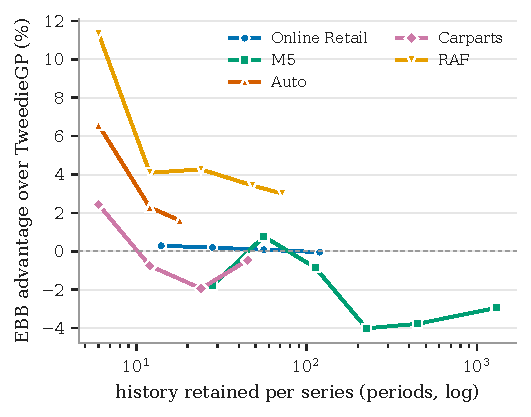
\includegraphics[width=0.98\linewidth]{figs/fig13_coldstart.pdf}
\caption{\textbf{Pooling pays when histories are short.} \EBB{}'s
mean-SPL advantage over TweedieGP (percent) against the history retained
per series at initialization; the evaluation span is fixed and the audited
structure and discount are unchanged. Full-length points reproduce
Table~\ref{tab:prob}.}
\label{fig:coldstart}
\end{figure}

\begin{figure*}[t]
\centering
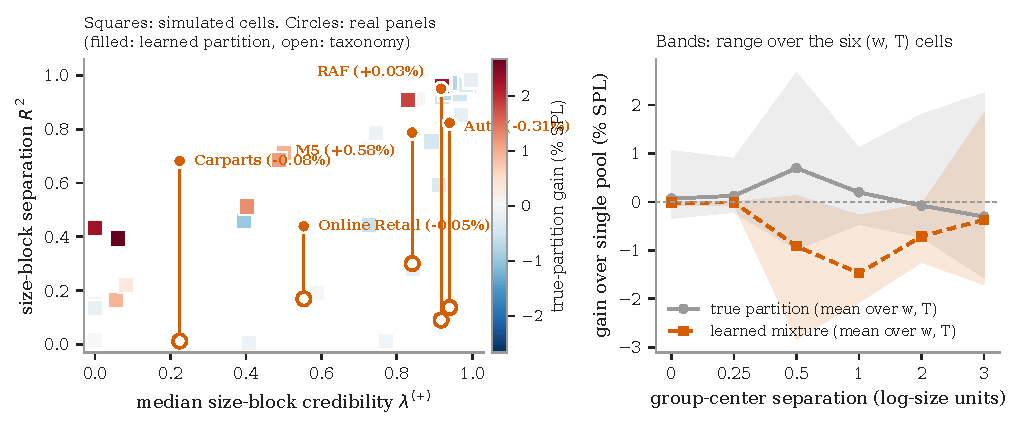
\includegraphics[width=0.98\textwidth]{figs/fig14_separation_surface.pdf}
\caption{\textbf{Room depends on separation as well as leverage, and the
real panels have little of it.} Left: each square is one cell of the
controlled grid (separation $\times$ discount $\times$ length, nine paired
replicates; occurrence separation scaled with size separation), placed at its median size-block credibility and at the share
of item log-size variance its true partition explains ($R^2$), colored by
the true partition's SPL gain over a single pool. Real panels are placed
at the same two coordinates, with $R^2$ measured under the learned
partition (filled) and under the objective-free ADI/CV$^2$ taxonomy (open);
labels give the learned partition's realized refinement gain. Right: the
true partition's gain and the learned mixture's gain against separation,
averaged over the six $(w,T)$ cells, with the range across cells shaded.
Room read within each panel's own forgetting regime is in
Table~\ref{tab:separation}.}
\label{fig:separation}
\end{figure*}

\paragraph{Where the room is, and whether it is collected.}
Figure~\ref{fig:separation} places the five panels on a surface that
varies leverage and group separation together. Each panel's size-block
separation is measured as the share of item log-size variance explained
by a partition, $R^2$, under its learned partition ($0.44$ to $0.95$) and
under the objective-free ADI/CV$^2$ taxonomy ($0.01$ to $0.30$); the
simulated cells carry the same statistic under their true labels. Read
within each panel's own forgetting regime (Table~\ref{tab:separation}), a
supplied true partition would earn between $-0.5\%$ and $+0.6\%$ on
Online Retail, M5, Auto, and RAF, and $1.7$ to $2.0\%$ on Carparts. The
learned partitions return $-0.05\%$, $+0.58\%$, $-0.31\%$, $+0.03\%$, and
$-0.08\%$: within the surface's range on the four panels without room,
and about two points short on the one panel with it. At Carparts's
coordinates the simulated learned mixture also loses ($-0.7\%$ to $-0.8\%$), and across the grid it is negative at every moderate
separation (Figure~\ref{fig:separation}, right), recovering the true
partition's return only when centers are two or more log-units apart and
histories are long. The earlier reading of Online Retail as the decisive
case rested on an envelope that pooled separations; resolved, its room is
at most $0.6\%$.

This separates the two explanations that aggregate results cannot. On
four panels the credibility weights and the separation together say there
is little to exploit, and the estimator's near-zero refinement gains are
the predicted outcome, not a failure. On Carparts the structure would pay
and the objective does not find it; that the same objective fails on
simulated panels at the same coordinates makes learnability, not the
bound, the binding constraint there. Corollary~\ref{cor:resolution}
bounds the prize; the surface says where the prize is nonzero.

\paragraph{Forgetting is an order of magnitude larger.}
Computed within a single selection surface under one definition---the
M5 surface at its selected discount---refining the pooling
structure is worth $+0.58\%$ of validation SPL, while discounting at the
same structure is worth $8.95\%$ for the global pool and $9.46\%$ for the
mixture. The asymmetry that motivates the paper survives at an order of
magnitude, and it survives on the one panel where refinement is
measurable at all.


\paragraph{A pre-fit screen.}
The surface answers the question ex post, with true labels; the
practical question is ex ante. On an expanded controlled grid
(separation, discount, length, occurrence rate, group size, imbalance;
$2{,}700$ panels), a closed-form score computed from the single-pool fit
alone, $\mathrm{med}_i(1-\lambda_i^{(+)})^2\,\hat\tau^2$, ranks the room a
true partition could earn with held-out AUC 0.71--0.71 for
the event ``gain above one percent''; a logistic screen on the same
fitting-window quantities reaches 0.84--0.83 when separation
levels, lengths, or random folds are held out and 0.68 when a
whole discount is held out, so the screen interpolates across regimes it
has seen and does not extrapolate across the discount
(Appendix~\ref{app:room}). Two facts bound the claim. 39\% of the
simulated single-pool fits collapse ($\hat\tau^2=0$) and half of the
large oracle gains occur there: escapes from a collapsed global fit,
which the resolution statistic flags, not returns to structure. And on
real series with a known partition injected---group offsets of up to two
log-units on Online Retail, Carparts, and M5, at the selected discount and
at $w=0.90$---the oracle partition never earns more than 0.4\%,
because a single pool absorbs the injected heterogeneity into
$\hat\tau^2$ and the items' own evidence takes over; the screen assigns
every such panel a probability below 0.17 of material room,
correctly, but the test checks rejections, not detections. The screen
therefore does what Corollary~\ref{cor:resolution} licenses and no more:
it identifies, from the fitting window, regimes where refinement cannot
pay materially.


% =========================================================================
\subsection{Accuracy and cost}\label{sec:accuracy}
% =========================================================================

\begin{table*}[t]
\centering
\caption{\textbf{Mean scaled pinball loss on five panels under two
protocols.} Fixed origin fits once and scores the full evaluation span;
walk-forward reveals one block at a time (seven days on the daily panels,
one month on the monthly ones), with every baseline refit per block and
\EBB{} updating sufficient statistics. The first row is the best of ten
classical, automatic, and static split-conformal baselines in each cell
(Online Retail: iETS / AutoTheta; M5: CP-Croston / CP-IMAPA; Auto: AutoARIMA / AutoARIMA; Carparts: CP-IMAPA / CP-IMAPA; RAF: CP-ADIDA / CP-ADIDA).
ACI-ADIDA is adaptive conformal inference on ADIDA; \EBB{} (rule) applies
the same adaptive layer to \EBB{} only where a validation-tail rule inside
the initialization window selects it, and is not ranked. Bold marks the
column's best ranked method. Full tables with all quantiles, coverage,
significance, and cost are in Appendix~\ref{app:demoted} and
Appendix~\ref{app:extra}.}
\label{tab:main}
\small
\setlength{\tabcolsep}{3.6pt}
\begin{tabular}{lrrrrrrrrrr}
\toprule
 & \multicolumn{5}{c}{Fixed origin} & \multicolumn{5}{c}{Walk-forward}\\
\cmidrule(lr){2-6}\cmidrule(lr){7-11}
Method & OR & M5 & Auto & Carp. & RAF & OR & M5 & Auto & Carp. & RAF\\
\midrule
Best classical or static-conformal baseline & 0.985 & 1.690 & 0.319 & 0.356 & 0.310 & 1.059 & 1.546 & 0.314 & 0.349 & 0.309\\
ACI-ADIDA & --- & --- & --- & --- & --- & 0.911 & \best{1.419} & 0.315 & 0.342 & 0.308\\
TweedieGP (per-series GP) & \best{0.884} & \best{1.623} & 0.298 & \best{0.321} & 0.276 & \best{0.853} & --- & 0.292 & \best{0.312} & 0.280\\
\midrule
\EBB{} & 0.885 & 1.671 & \best{0.294} & 0.323 & \best{0.268} & 0.854 & 1.485 & \best{0.291} & 0.315 & \best{0.268}\\
\EBB{} (calibration by rule) & --- & --- & --- & --- & --- & 0.854 & 1.379 & 0.290 & 0.315 & 0.268\\
\bottomrule
\end{tabular}
\end{table*}

Table~\ref{tab:main} reports the comparison that a practitioner would
make. At fixed origin, \EBB{} attains the lowest mean SPL on Auto and RAF,
by $1.6\%$ and $3.0\%$ over the official TweedieGP implementation, both
significant; TweedieGP attains it on Online Retail, Carparts, and M5, by
$0.05\%$, $0.5\%$, and $2.9\%$, of which only the M5 margin is
significant. Against every other comparator \EBB{} is best on all five
panels, by $10.1\%$ over iETS on Online Retail and $1.2\%$ over
CP-Croston on M5 (Appendix~\ref{app:demoted}, Table~\ref{tab:prob};
significance in Appendix~\ref{app:extra}, Table~\ref{tab:spl-significance}).
Under strict walk-forward updating the picture repeats for the
uncalibrated methods: \EBB{} leads on Auto and RAF, TweedieGP on Online
Retail and Carparts by $0.2\%$ and $0.8\%$, and per-series paired tests
cannot separate the two on three of the four panels where both run.
Adaptive conformal inference on ADIDA leads M5 by $4.4\%$; the same layer
applied to \EBB{} lowers its M5 loss from $1.485$ to $1.379$, $2.9\%$
below ACI-ADIDA, but degrades Online Retail and RAF, so whether to apply
it is itself selected on the validation tail. The rule applies the layer
on M5 and Auto, withholds it elsewhere, matches the ex-post better variant
on four of five panels, and leaves \EBB{} (rule) within $0.8\%$ of the
best competing method on every panel (Appendix~\ref{app:demoted},
Tables~\ref{tab:wfprob}--\ref{tab:regret}; Appendix~\ref{app:extra},
Table~\ref{tab:aci-rule}).


\begin{figure}[t]
\centering
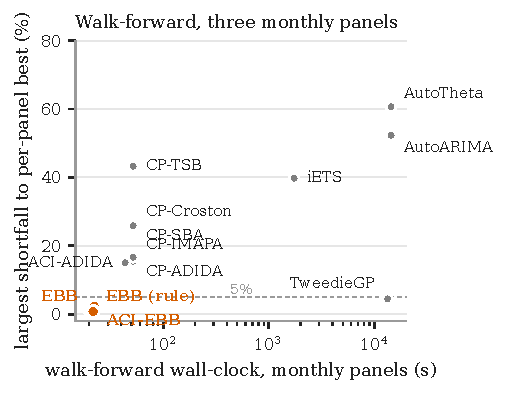
\includegraphics[width=0.98\linewidth]{figs/fig12b_frontier_wf.pdf}
\caption{\textbf{Largest shortfall against cost under walk-forward
updating.} Each point is one method on the three monthly panels, on which
every method has a measured wall-clock: $y$ is its largest mean-SPL
shortfall to the per-panel best, $x$ the total walk-forward wall-clock
(TweedieGP uses twelve workers, every other method one process). The
fixed-origin counterpart and the full regret tables are in
Appendix~\ref{app:demoted}.}
\label{fig:frontier}
\end{figure}

Figure~\ref{fig:frontier} summarizes both protocols by the largest
shortfall to the per-panel best against measured cost. \EBB{} and
TweedieGP are the only methods within five percent of the best competitor
everywhere (\EBB{} at most $3.0\%$ at fixed origin and $4.6\%$ under
walk-forward updating; TweedieGP $3.1\%$ and $4.5\%$); every other method
is at least $15\%$ behind on some panel. The two differ in cost by one to
three orders of magnitude: TweedieGP refits per-series variational GPs at
every update, so its walk-forward runs took between $36$ minutes and
$2.4$ hours with twelve workers and project to about $51$ hours on M5,
whereas \EBB{} completes each of the five walk-forward runs in under $40$
seconds on one core, updating sufficient statistics in closed form
(Appendix~\ref{app:efficiency}). Point forecasts are competitive but not
uniformly best (Appendix~\ref{app:point}).

% =========================================================================
\subsection{Two evaluation cautions}\label{sec:cautions}
% =========================================================================

The first caution concerns the probabilistic baseline: \emph{the choice of conformal construction matters more here than
the choice of forecaster}: making the wrapper adaptive
\citep{gibbs2021} improves ADIDA's mean SPL from $1.1576$ to $0.9108$, a
$21\%$ gain that is more than three times the remaining gap to \EBB{}.
Static split-conformal wrappers are the standard probabilistic baseline in
this literature; on this evidence they understate what conformal
prediction can do on intermittent panels, and comparisons drawn against
them---including earlier versions of our own---are correspondingly
generous.
The second caution concerns point metrics. The all-zero forecast attains
the lowest MAE on three of five panels and, in the controlled study, a
known-correct partition is reported as harmful by MAE while improving
every proper scoring rule (Appendix~\ref{app:demoted},
Table~\ref{tab:sanity}); absolute-error criteria should not be the sole
basis for comparing intermittent-demand forecasters, and we use them
only as diagnostics.
